\documentclass[a4]{article}

\usepackage{fullpage}
\usepackage{graphicx}
\usepackage{tikz}
  \usetikzlibrary{arrows}
\usepackage{listings}
\usepackage{theorem}
\usepackage{url}
\usepackage{xspace}
\usepackage{amssymb}
\usepackage{xtab}
\usepackage{todonotes}
\usepackage{fancyvrb}

%\newcommand{\todo}[1]{{\bf [TODO: }\textit{#1}{\bf ]}}
\newcommand{\remark}[1]{{\bf [RemarkKVH: }\textit{#1}{\bf ]}}
\newcommand{\remarktmb}[1]{{\bf [RemarkTMB: }\textit{#1}{\bf ]}}

\newcommand{\EIS}{\textsf{EIS}\xspace}
\newcommand{\IILang}{\textsf{IILang}\xspace}

\newcommand{\Goal}{\textsc{GOAL}\xspace}
\newcommand{\Jason}{\textsc{Jason}\xspace}
\newcommand{\twoAPL}{\textsc{2APL}\xspace}
\newcommand{\Jadex}{\textsc{Jadex}\xspace}

\newtheorem{example}{Example}





\begin{document}

\title{\bf 
Guide for \EIS-0.3
}

\author{Tristan Behrens}
\date{\today}

\maketitle

\section{INTRODUCTION}

This document's intent is 1. to give an overview on how to integrate \EIS with your project and 2. how to \emph{EISify} your own or third-party environments, that is making it EIS-compatible. This paper is supposed to be a document complemental to the \EIS-javadoc. Things that you will not find
in this document, you will find in the javadoc. For the general motivation behind \EIS please refer
to our technical report\footnote{\url{http://www.in.tu-clausthal.de/fileadmin/homes/techreports/ifi0909behrens.pdf}}.

This document consists of
\begin{enumerate}
\item a \emph{platform guide} that explains how to connect your APL platform to \EIS, and
\item a \emph{interface guide} that explains how to make your environments \EIS-compatible.
\end{enumerate}

\subsection{Building, Installing and Linking}

We can assume that you have already successfully downloaded \EIS from sourceforge. 
There are two ways to link \EIS to your project: 1. either you manually add the jar-files contained in 
the software-package to the class-path of your project, or 2. you install \EIS via Maven\footnote{\url{http://maven.apache.org/}}
and add it as a dependency. We assume that you are familiar with adding jars to the class-path. Thus, in the following, we
will only elaborate on using Maven.

When downloading the software-package you will find a couple of jars in the zip-file:
\begin{itemize}
\item\texttt{eis-0.3.jar} contains the compiled classed, constituting the main dependency,
\item\texttt{eis-0.3-javadoc.jar} contains the javadoc generated from the classes, which is very useful, and
\item\texttt{eis-0.3-sources.jar} contains the sources of \EIS, which is useful for source-attachments to you project.
\end{itemize}

To build \EIS you have to have Maven installed (see the Maven-homepage for instructions). Navigate to
the folder that contains the file \texttt{pom.xml} and run this command:
\begin{quote}
\texttt{mvn install}
\end{quote}
This will compile \EIS, run some JUnit tests, bundle the compiled classes into a single jar-file, generate a javadoc and install 
everything to your local Maven-repository. Note at this point, that the \texttt{target/}-folder will now contain the three jars
mentioned above.

Now you can add \EIS as a dependency to your \texttt{pom.xml}:
\begin{Verbatim}[frame=single]
<dependencies>
  <dependency>
    <groupId>apleis</groupId> 
    <artifactId>eis</artifactId> 
    <version>0.3</version> 
    <scope>compile</scope>
  </dependency>
  ...
</dependencies>
\end{Verbatim}
The dependency will then automatically be resolved, when you compile your project.

\subsection{About \EIS-Versions}

\EIS versioning works as follow. The first digit in the version-number is \texttt{0}. The second digit
indicates the major revision (currently \texttt{3}). A major revision is characterized by the introduction of new features.
Additionally, for minor revisions, the SVN-revision-number is stored in the manifest of the \EIS
jar-file. This number can easily be accessed by unzipping the jar-file. Of course, to do so, you are free
to use any means. In a UNIX-like environment you can do this in the console:
\begin{Verbatim}[frame=single]
unzip -c target/eis-0.3.jar META-INF/MANIFEST.MF
\end{Verbatim}
Which would yield something like this:
\begin{Verbatim}[frame=single]
Manifest-Version: 1.0
Archiver-Version: Plexus Archiver
Created-By: Apache Maven
Built-By: tristanbehrens
Build-Jdk: 1.6.0_22
SCM-Revision: 67
\end{Verbatim}
The number \texttt{67} indicates the revision.

\subsection{Interface Meta-Model}

Fig.~\ref{FIGENVMODEL} shows the \EIS interface meta-model. We define that the overall system consists
of these components:
\begin{itemize}
\item \emph{agents}, 
\item the \emph{platform} that manages and executes agents,
\item the  \emph{environment management system} that facilitates managing the environment,
\item the \emph{agents-entities system} that connects agents to controllable entities,
\item the \emph{environment querying system} that allows for querying the environment-interface for statistics, and
\item the \emph{environment model} that represents the environment itself.
\end{itemize}

\begin{figure}[h]
\begin{center}
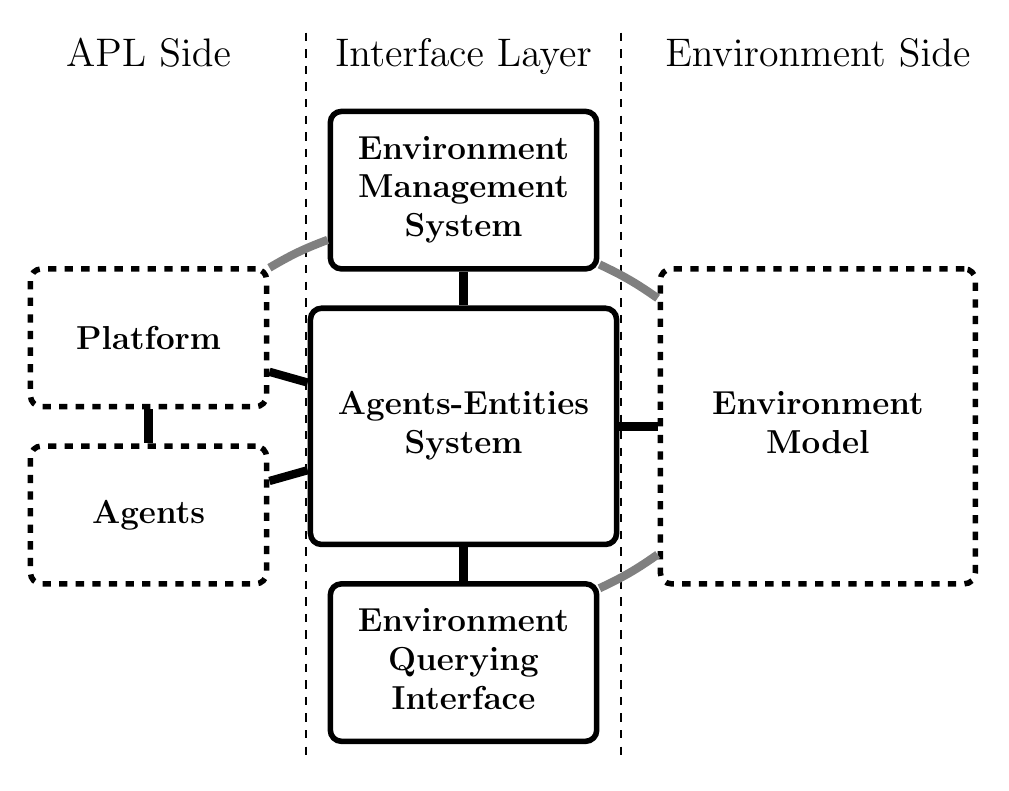
\begin{tikzpicture}[line width=2pt,scale=1]\large
%\draw[-,dashed,line width=1pt] (4,5) to (4,-2.75);
\node(text1) at(0,4.75){\Large APL Side};
\node(text1) at(8.5,4.75){\Large Environment Side};
\node(text1) at(4,4.7){\Large Interface Layer};
\draw[-,dashed,line width=1pt] (2,5) to (2,-4.25);
\draw[-,dashed,line width=1pt] (6,5) to (6,-4.25);

\node[rectangle, draw=black,fill=white,rounded corners, minimum width=3cm, minimum height = 2cm] (envman) at (4,3){\bf \begin{tabular}{ccc}Environment\\Management\\System\end{tabular}};
\node[rectangle, draw=black,fill=white,rounded corners, minimum width=3cm, minimum height = 1.75cm, dashed] (platform) at (0,1.125){\bf Platform};
\node[rectangle, draw=black,fill=white,rounded corners, minimum width=3cm, minimum height = 1.75cm, dashed] (agents) at (0,-1.125){\bf Agents};
\node[rectangle, draw=black,fill=white,rounded corners, minimum width=3cm, minimum height = 3cm] (eis)  at (4,0) {\bf \begin{tabular}{ccc}Agents-Entities\\System\end{tabular}};
\node[rectangle, draw=black,fill=white,rounded corners, minimum width=4cm, minimum height = 4cm, dashed] (env) at (8.5,0){\bf \begin{tabular}{ccc}Environment\\Model\end{tabular}};
\node[rectangle, draw=black,fill=white,rounded corners, minimum width=3cm, minimum height = 2cm] (envquer) at (4,-3){\bf \begin{tabular}{ccc}Environment\\Querying\\Interface\end{tabular}};

\draw[-,line width=3pt] (envman) to (eis);
\draw[-,line width=3pt] (eis) to (agents);
\draw[-,line width=3pt] (platform) to (agents);
\draw[-,line width=3pt] (platform) to (eis);
\draw[-,line width=3pt] (eis) to (env);
\draw[-,line width=3pt,bend right=5,color=gray] (envman) to (platform);
\draw[-,line width=3pt,bend right=5,color=gray] (env) to (envman);
\draw[-,line width=3pt] (eis) to (envquer);
\draw[-,line width=3pt,bend right=5,color=gray] (envquer) to (env);

\end{tikzpicture}
\end{center}
\caption{The interface meta-model. We have three different layers. The platform and its agents live on the APL side. The environment management system, that facilitates the
manipulation of the environments executional state, the
agents-entities system, that connects agents to controllable entities, and the environment-querying system, that allows
for querying the environment and the environment interface for data, all live on the interface layer. And the environment model lives on the environment side.}
\label{FIGENVMODEL}
\end{figure}

\subsection{Interface Intermediate Language}

The  Interface Intermediate Language (\IILang) consists of 1. \emph{data containers} (e.g. actions and percepts), 2. \emph{parameters}
to those containers, and 3. \emph{environment states} (see Fig.~\ref{FIG:IILANG}). 
Members of the \IILang are stored as abstract syntax trees formed by Java-objects, which can be printed
either in an XML- or in an logic-programming style for the sake of readability.

Any token from the \IILang can be rendered to a textual representation by invoking the methods
\texttt{toString()}, \texttt{toXML()}, or \texttt{toProlog()} alternatively.
\texttt{toXML()} yields a XML-representation and \texttt{toProlog()} yields a Prolog-like one.
\texttt{toString()} on the other hand yields the standard representation, which is XML per default.
This can be changed during runtime by setting the static variable \texttt{toProlog} of 
\texttt{eis.iilang.IILangElement}, like this
\begin{Verbatim}[frame=single]
IILangElement.toProlog = true;
\end{Verbatim}

Parameters are: identifiers, numbers, truth-values, functions over parameters, and lists of parameters.
These are the Java-classes representing parameters:
\begin{itemize}
\item\texttt{eis.iilang.Identifier} represents an identifier,
\item\texttt{eis.iilang.Numeral} represents a number,
\item\texttt{eis.iilang.TruthValue} represents a truth-value,
\item\texttt{eis.iilang.Function} represents a function over parameters, and
\item\texttt{eis.iilang.ParameterList} represents a list of parameters.
\end{itemize}

Parameters are supposed to be instantiated by calling one constructor, like this:
\begin{Verbatim}[frame=single]
Identifier id = new Identifier("name");
\end{Verbatim}
See the javadoc for a full overview on the constructors.

\begin{figure}[h]\centering
\tikzstyle{node}=[rectangle,draw=black,minimum width =2.5cm,minimum height = 0.75cm]
\begin{tikzpicture}
\node[node] (NA) at (0,-0.75) {\texttt{IILElement}};% at (0,0);
\node[node] (NB1) at (4,1) {\texttt{DataContainer}};
\node[node] (NB2) at (4,-2.5) {\texttt{Parameter}}; 
\node[node] (NC1) at (8,1.5) {\texttt{Action}};
\node[node] (NC2) at (8,0.5) {\texttt{Percept}};
\node[node] (NC3) at (8,-0.5) {\texttt{Identifier}};
\node[node] (NC4) at (8,-1.5) {\texttt{Numeral}};
\node[node] (NC5) at (8,-2.5) {\texttt{TruthValue}};
\node[node] (NC6) at (8,-3.5) {\texttt{ParameterList}};
\node[node] (NC7) at (8,-4.5) {\texttt{Function}};
\draw[-] (NA) to (NB1);
\draw[-] (NA) to (NB2);
\draw[-] (NB1) to (NC1);
\draw[-] (NB1) to (NC2);
\draw[-] (NB2) to (NC3);
\draw[-] (NB2) to (NC4);
\draw[-] (NB2) to (NC5);
\draw[-] (NB2) to (NC6);
\draw[-] (NB2) to (NC7);
\end{tikzpicture}
\caption{The inheritance relation of the IIL-elements. Actions and percepts are data-containers. Each data-container consists of a name and an ordered collection of parameters. Each parameter is either an identifier, a numeral, a list of parameters or a function of parameters.}
\label{FIG:IILANG}
\end{figure}

Data containers are: actions that are performed by agents, and
percepts sent by the environment-interface and received by agents or percepts as results of actions.

Each of these data containers consist of (1) a name, and (2) a set of parameters.
Here are the respective classes:
\begin{itemize}
\item\texttt{eis.iilang.Action} represents an action.
\item\texttt{eis.iilang.Percept} is a percept.
environment.
\end{itemize}

Like parameters, data containers are supposed to be instantiated using a constructor, like this:
\begin{Verbatim}[frame=single]
Action act = new Action("goto", new Identifier("node1"));
\end{Verbatim}

Again, please refer to the javadoc for a full overview of the constructors.

\subsection{Environment Management System}

The environment management system (EMS, as shown in Fig.~\ref{FIG:EMS}) is the component of \EIS that facilitates managing the
state of execution of the environment(-interface). Basically this is a finite state machine that encodes the different
states of the environment(-inferface) and the possible state transitions.

The state if represented by the enum \texttt{eis.iilang.EnvironmentState}.
We have several states:
\begin{itemize}
\item\texttt{EnvironmentState.INITIALIZING}:
as soon as the environment-interface is instantiated it is initializing. 
\item\texttt{EnvironmentState.PAUSED}: as soon as the connection to the environment has been
established the environment-interface is in the \texttt{PAUSED}-state, that is entering the \texttt{PAUSED}-state
ends the initializing-phase.
\item\texttt{EnvironmentState.STARTED}: the environment is running. Only in this state actions are accepted and 
percepts are provided. 
\item\texttt{EnvironmentState.KILLED}: the environment is killed. The environment-interface  and its resources can be released.
\end{itemize}

The state transitions on the other hand are these:
\begin{itemize}
\item \texttt{INITIALIZING} to \texttt{INITIALIZING} via \texttt{init(...)}: you can further set up the environment-interface by providing initialization parameters, which is facilitated by calling the \texttt{init(...)}-method with the respective parameters. Note that we assume what calling that method is not obligatory, which in turn implies that there needs to
be a default-initialization for all specific environment-interfaces.
\item \texttt{INITIALIZING} to \texttt{PAUSED} via \texttt{*}: we assume that there will be a process of connecting
to an environment right after initializing the specific environment interface. As soon as that connection is established
the state is supposed to be \texttt{PAUSED}. We denote that process of connecting with \texttt{*}.
\item \texttt{INITIALIZING} to \texttt{KILLED} via \texttt{kill()}: this kills the environment interface, before even the
connection to the environment was established.
\item \texttt{PAUSED} to \texttt{STARTED} via \texttt{start()}: this starts the execution.
\item \texttt{PAUSED} to \texttt{KILLED} via \texttt{kill()}: this kills the environment interface.
\item \texttt{STARTED} to \texttt{PAUSED} via \texttt{pause()}: this pauses the execution.
\item \texttt{STARTED} to \texttt{KILLED} via \texttt{kill()}: this kills the environment interface.
\end{itemize}

Every time such a state transition occurs the connected listeners are supposed to be notified about that event. To that end, when the
state is changed the method  \texttt{handleStateChange(...)} must be called for all registered environment-listeners (see below).
The default implementation already handles the state-transitions, it throws an exception if an invalid state-transition
is tried, and automatically notifies all listeners about the state-change if it was successful.

On top of that the current state can be queried via the \texttt{getState()}-method, which should return an instance of
\texttt{eis.iilang.EnvironmentState}. Again the default implementation already handles this.

\begin{figure}[h]\centering
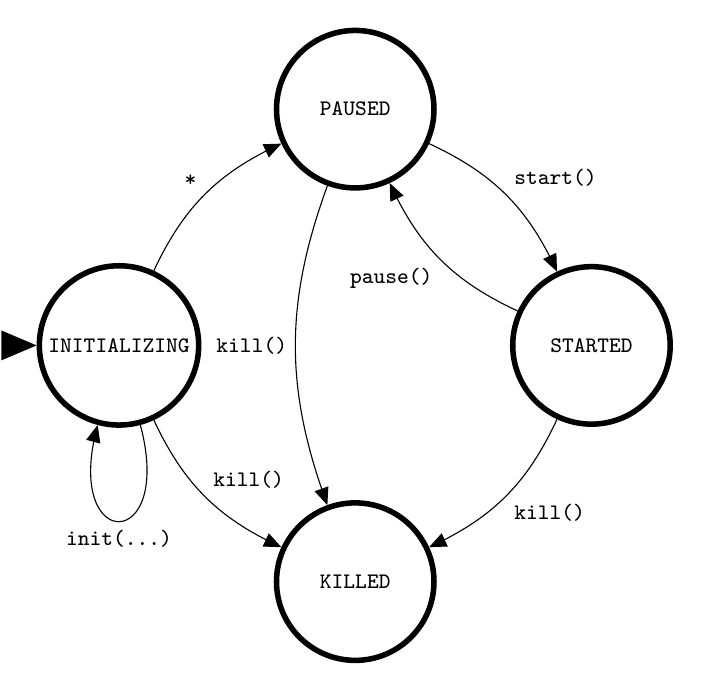
\begin{tikzpicture}[>=triangle 45]\footnotesize
\tikzstyle{state}=[draw=black,circle,line width=2pt,minimum width=2cm]
\node[state] (IN) {\texttt{INITIALIZING}};
\node[state] (PA) at (3,3) {\texttt{PAUSED}};
\node[state] (ST) at (6,0) {\texttt{STARTED}};
\node[state] (KI) at (3,-3) {\texttt{KILLED}};
\draw[->,loop below] (IN) to node[below] {\texttt{init(...)}} (IN);
\draw[->,line width=2pt] (-1.125,0) to (IN);
\draw[->,bend left=20] (IN) to node[above left] {\texttt{*}} (PA);
\draw[->,bend right=20] (IN) to node[above right] {\texttt{kill()}} (KI);
%\draw[->,bend left=20] (PA) to node[below right] {\texttt{RESET}} (IN);
\draw[->,bend left=20] (PA) to node[above right] {\texttt{start()}} (ST);
\draw[->,bend left=20] (ST) to node[below left] {\texttt{pause()}} (PA);
\draw[->,bend left=20] (ST) to node[below right] {\texttt{kill()}} (KI);
\draw[->,bend right=20] (PA) to node[left] {\texttt{kill()}} (KI);
%\draw[->,bend left=20] (ST) to node[below] {\texttt{RESET}} (IN);

\end{tikzpicture}
\caption{Different states of the environment interface and state transitions.}
\label{FIG:EMS}
\end{figure}

\subsection{Agents and Controllable Entities}

An important concept of \EIS is the separation of concerns, that is the distinction between
1. agents that are software structures that act as percept-processors and action-generators on the platform side,
and 2. controllable entities that are software structures that act as percept-generators and action-processors on the environment side. The connections between agents and controllable entities is made possible by the 
\emph{agents-entities-relation}, that in its essence a subset of the crossproduct of the set of agents and the set of entities. 

The environment-interface in general is very agnostic about the internal structure of both agents and entities, and thus stores them internally represented only as strings (see Fig.~\ref{AGENREL}). These strings are then associated in the agents-entities-relation. How, we will show later. Acting an perceiving is then to be mapped respectively.

\begin{figure}[h]
\begin{center}
\begin{tikzpicture}[line width=2pt,scale=1]\large
\tikzstyle{aeid}=[draw=black,circle, minimum size = 0.75cm, line width=1pt, inner sep=0]
\tikzstyle{object}=[draw=black,circle, minimum size = 1cm, line width=1.5pt, inner sep=0]
\tikzstyle{conn}=[draw=black,line width=1.5pt]
\tikzstyle{connthin}=[draw=black,line width=1pt]

%\draw[-,dashed,line width=1pt] (4,5) to (4,-2.75);
\node(text1) at(0,3.75){\Large APL Side};
\node(text1) at(8.5,3.75){\Large Environment Side};
\node(text1) at(4,3.7){\Large Interface Layer};
\draw[-,dashed,line width=1pt] (2,4) to (2,-2.75);
\draw[-,dashed,line width=1pt] (6,4) to (6,-2.75);

\node[] (ag1) at (0,2) {\bf Agent};
\node[] (ag2) at (0,0) {\bf Agent};
\node[] (ag3) at (0,-2) {\bf Agent};

\node[aeid] (aid1) at (3,1.25) {Id};
\node[aeid] (aid2) at (3,0) {Id};
\node[aeid] (aid3) at (3,-1.25) {Id};

\node[aeid] (eid1) at (5,1.5) {Id};
\node[aeid] (eid2) at (5,0.5) {Id};
\node[aeid] (eid3) at (5,-0.5) {Id};
\node[aeid] (eid4) at (5,-1.5) {Id};

\node[] (en1) at (8,2) {
\includegraphics[width=0.75cm]{robot}};
\node[] (en2) at (8,0.75) {
\includegraphics[width=0.75cm]{robot}};
\node[] (en3) at (8,-0.75) {
\includegraphics[width=0.75cm]{robot}};
\node[] (en4) at (8,-2) {
\includegraphics[width=0.75cm]{robot}};

\draw[conn, bend left=10] (ag1) to (aid1);
\draw[conn] (ag2) to (aid2);
\draw[conn, bend right=10] (ag3) to (aid3);

\draw[conn, bend right=10] (en1) to (eid1);
\draw[conn, bend right=5] (en2) to (eid2);
\draw[conn, bend left=5] (en3) to (eid3);
\draw[conn, bend left=10] (en4) to (eid4);

\draw[connthin] (aid1) to (eid1);
\draw[connthin] (aid2) to (eid2);
\draw[connthin] (aid2) to (eid3);
\draw[connthin] (aid3) to (eid4);

\end{tikzpicture}

\end{center}
\caption{The agent entities-relation. Agents are percept processors and action generators that live on the APL side. Controllable entities are percept generators and action processors and live on the environment side. Both agents and controllable entities are represented via identifiers on the interface layer.}
\label{AGENREL}
\end{figure}



\newpage
\section{EIS PLATFORM GUIDE}

In this section we will provide an tutorial about how to integrate \EIS into your (agent programming) platform. 
We suppose that you have already downloaded the complete package as described earlier. 

\subsection{Linking and Loading}

The first thing that you have to do is adding \EIS to the class-path of your project. We have already described this earlier.
The next thing that you have to do is to employ the jar-loading-mechanism that comes with \EIS. 
Specific environment-interfaces are distributed as jar-files. 
The class \texttt{eis.EILoader} should be used to load an environment-interface from a jar-file and instantiate it.
Use the method \texttt{fromJarFile}:
\begin{Verbatim}[frame=single]
EnvironmentInterfaceStandard ei = null;
try {
    ei = EILoader.fromJarFile(new File(jarFileName));
} catch (IOException e) {
    // TODO handle the exception
}
\end{Verbatim}
Note that you have to handle exceptions that are potentially thrown by the invocation of the method. 
Possible causes for failure could be that the file does not exist or that the version (\EIS has a versioning-system) does not match the required one.

Alternatively, that is if the environment-interface is already in the class-path you can use the
method \texttt{fromClassName}.

\subsection{Attaching Listeners for Interface-Platform Communication}

Communication with \EIS-interfaces is facilitated 1. by calling specific methods, and 2. by handling callbacks
that the respective interfaces raise. \EIS provides two listener-interfaces: 
\begin{itemize}
\item \texttt{eis.EnvironmentListener} for handling state changes of the interface, and
\item \texttt{eis.AgentListener} for handling percepts-as-notifications.
\end{itemize}

On the platform side you should provide classes that implement these interfaces.
When you run the system you are supposed to register instances of these classes to the instantiated environment-interface, using these methods of \texttt{eis.EnvironmentInterfaceStandard}:
\begin{itemize}
\item \texttt{attachEnvironmentListener(EnvironmentListener listener)} for attaching an environment-listener, and
\item \texttt{attachAgentListener(String agent, AgentListener listener)} for attaching an agent-listener.
\end{itemize}

You can attach as many listeners as you like. Note also, that you can unregister any listener during runtime using these methods:
\begin{itemize}
\item \texttt{detachEnvironmentListener(EnvironmentListener listener)} for detaching an environment-listener, and
\item \texttt{detachAgentListener(AgentListener listener)} for detaching an agent-listener.
\end{itemize}

\subsection{Managing the Environment State}

In order to receive notifications about environment-state changes you have to implement the \texttt{eis.EnvironmentListener} interface and register at least one instance of a respective class via
\texttt{attachEnvironmentListener}. Every time the state changes, the environment-interface will
invoke this method, which you have to implement in order to react to these changes:
\begin{quote}
\texttt{void handleStateChange(EnvironmentState newState);}
\end{quote}
Note that you can query the state at any time by invoking this method of \texttt{eis.EnvironmentInterfaceStandard}:
\begin{quote}
\texttt{EnvironmentState getState();}
\end{quote}

To manipulate the state you have access to this set of methods:
\begin{itemize}
\item\texttt{void init(Map<String,Parameter> parameters) throws ManagementException},
\item\texttt{void start() throws ManagementException},
\item\texttt{void pause() throws ManagementException}, and
\item\texttt{void kill() throws ManagementException}.
\end{itemize}

You can initialize an environment-interface by calling \texttt{init} with a set of key-value pairs.
Note that all these methods raise a \texttt{ManagementException} in the case that the respective
state transition is not supported. To query whether a state-transition is supported at all you can 
employ this set of methods:
\begin{itemize}
\item\texttt{boolean isInitSupported()} returns \texttt{true} if \texttt{init(...)} is supported,
\item\texttt{boolean isStartSupported()}  returns \texttt{true} if \texttt{start()} is supported,
\item\texttt{boolean isPauseSupported()}  returns \texttt{true} if \texttt{pause()} is supported, and
\item\texttt{boolean isKillSupported()}  returns \texttt{true} if \texttt{kill()} is supported.
\end{itemize}
		
	
\subsection{Setting up Agents, Acting and Perceiving}

Now that you have successfully instantiated an environment-interface you have to register your agents.
Since \EIS is very agnostic when it comes to the type/structure/architecture of your agents you only have to
register your agents by providing their names. The reason for this is the desired generality. 
So let us assume that you have some agent, which is represented by its name.
You can register the agent like this:
\begin{Verbatim}[frame=single]
String agentName = ... ; // the name of your agent
try {
    ei.registerAgent(agentName);
} catch (AgentException e) {
  // TODO handle the exception
}
\end{Verbatim}

Again, you have to handle possible exceptions. 
The invocation fails if an agent with the same name has already registered.
You can also unregister an agent if you want to cut it off from the environment-interface:
\begin{Verbatim}[frame=single]
try {
    ei.unregisterAgent(agentName);
} catch (AgentException e) {
  // TODO handle the exception
}
\end{Verbatim}
Here the invocation fails if the agent has not been registered to the interface.

The next thing we are going to do is associating agents with entities.
Assuming that you know that there is an entity with the name \texttt{"car1"}, you can make your agent control it like this:
\begin{Verbatim}[frame=single]
try {
    ei.associateEntity(agentName, "car1");
} catch (RelationException e) {
  // TODO handle the exception
}
\end{Verbatim}

The invocation could fail, so you have to handle the exception. Note that this a very naive way to associate your agent
with an entity, because it assumes that you know the name of the entity beforehand. 
You can however query the interface for all free entities and associate your agent with the first one:
\begin{Verbatim}[frame=single]
LinkedList<String> ens = ei.getFreeEntities();
try {
    ei.associateEntity(agentName, ens.removeFirst());
} catch (RelationException e) {
  // TODO handle the exception
}
\end{Verbatim}
Which policy you apply here is your decision. There are more methods for manipulating the agents-entities-relationship
(see the javadoc). Note that you can also query the type of an entity with the method \texttt{getType}. This could be useful
for example if you want to instantiate different types of agents for different types of entities.

Now that you have your agent registered and associated with an entity, or you have already iterated the process and associated
several agents with several entities, you want to make them act and perceive. Acting is quite simple. You have to invoke
the method \texttt{performAction} like this:
\begin{Verbatim}[frame=single]
Action action = ... // this has to be an EIS-action
try {
    Vector<Percept> ps = eis.performAction(agentName, action);
} catch (ActException e) {
  // TODO handle the exception
} catch (NoEnvironmentException e) {
  // TODO handle the exception
}
\end{Verbatim}
The action must be an instance of \texttt{eis.iilang.Action}. You could for example instantiate an action like this:
\begin{Verbatim}[frame=single]
Action action = new Action("goto", new Ident("up"));
\end{Verbatim}
It might be necessary to implement a mapping from your definition of what an action is to \EIS-actions.
Note that performing an action could return a percept. This is necessary for active sensing. 
Make sure that such return-values are handled properly.

Note that you can sometimes (depending on the environment-interface) associate a single agent with several entities.
This can be reflected by \texttt{performAction} that accepts an optional array of strings 
(vararg language feature\footnote{\url{http://java.sun.com/developer/JDCTechTips/2005/tt0104.html}}) as the third parameter. 
The array should contain a subset of the set of entities that are associated with the agent: 
\begin{Verbatim}[frame=single]
try {
  Vector<Percept> ps = eis.performAction(agentName, action,"entity1","entity2");
} catch (ActException e) {
  // TODO handle the exception
} catch (NoEnvironmentException e) {
  // TODO handle the exception
}
\end{Verbatim}
If the array is empty, all
entities will be taken into account. Note that you can determine the source (e.g. the entity) of each percept via the
\texttt{getSource}-method.

You definitely are advised to handle the exceptions. \texttt{NoEnvironmentException} is thrown if the environment-interface
is not properly connected to an environment. \texttt{ActException} is thrown if the action could not be executed. Possible
reasons for that are reflected by the type of the exception:
\begin{Verbatim}[frame=single]
try {
  ei.performAction(agentName, action,entities);
} catch (ActException e) {
  if( e.type == NOTYPE ) {
    // TODO handle the exception
  } else if( e.type == NOTREGISTERED ) {
    // TODO handle the exception
  } else if( e.type == NOENTITIES ) {
    // TODO handle the exception
  } else if( e.type == WRONGENTITY ) {
    // TODO handle the exception
  } else if( e.type == WRONGSYNTAX ) {
    // TODO handle the exception
  } else if( e.type == FAILURE ) {
    // TODO handle the exception
  }
} catch(NoEnvironmentException e) {
  // TODO handle the exception
}
\end{Verbatim}

The type \texttt{NOTSPECIFIC} denotes that the type of the exception has not been indicated specifically. 
Although we expect  more detailed information about why the method has failed, we do not enforce this.
\texttt{NOTREGISTERED} indicates that the agent has not registered to the environment-interface.
\texttt{NOENTITIES} on the other hand communicates that the agent has no associated entities.
\texttt{WRONGENTITY} denotes that at least one of the provided entities is not associated with the agent.
\texttt{NOTSUPPORTEDBYTYPE} indicates that the type of the entity does not support the execution of the action.
\texttt{WRONGSYNTAX} indicates that the syntax of the action is wrong. 
That is the case when the name of the action is not available and when the parameters do not match (number of parameters or their types and structure).
And \texttt{FAILURE} indicates that the action has failed although it matched all mentioned requirements. 
For example \texttt{goto(up)} could fail if the path is blocked in the respective direction.
 
Now let us talk percepts. There is a method to retrieve all percepts. This has been shown to be very useful for some APL platforms.
You can do this:
\begin{Verbatim}[frame=single]
try {
  LinkedList<Percept> percepts = ei.getAllPercepts(agentName);
  // TODO process the percepts
} catch (PerceiveException e) {
  // TODO handle the exception
} catch (NoEnvironmentException e) {
  // TODO handle the exception
}
\end{Verbatim}
After the invocation you have to make sure that the percepts are processed in a proper manner. 
Also a \texttt{PerceiveException} is thrown if perception fails, that is if the agent is not registered or has no associated
entities. An instance of \texttt{NoEnvironmentException} is thrown if there is no environment. Similar
to \texttt{performAction} the method \texttt{getAllPercepts} supports a vararg for restricting the call to a subset of the
associated entities.

Now let's talk about the third and final way to get percepts from the environment-interface: percepts-as-notifications.
\EIS supports sending percepts to the agents on special occasions without a request to do so. That is, environments
sending percepts. 
In order to allow your agents to receive such percepts, your platform has to implement the interface \texttt{eis.AgentListener} and its method \texttt{handlePercept(String agent, Percept percept)}. 
Furthermore you have to register the listener to the environment-interface.
The string \texttt{agent} of the \texttt{handlePercept}-method indicates the recipient of the percept \texttt{percept}.
Note that it is your responsibility to make sure that the percept is passed to the respective agent.

You can establish percepts-as-notifications like this:
\begin{Verbatim}[frame=single]
class YourPlatform implements AgentListener {

  EnvironmentInterface Standard ei;
  
  ...

  public void init() {
    eis.attachAgentListener(agentName, this);
  }

  public void handlePercept(String agent, Percept percept) {
    // TODO pass the percept to the agent
  }

}
\end{Verbatim}

Now we will discuss \emph{environment-events}. Such events are generated if 1. the set of entities changes or is modified, an 2. if the executional-state of the environment changes. Again you have to implement the interface 
\texttt{eis.EnvironmentListener} and its
methods: 
\begin{Verbatim}[frame=single]
class YourPlatform implements EnvironmentListener {

  EnvironmentInterface Standard ei;
  
  ...

  public void init() {
    eis.attachEnvironmentListener(this);
  }

  public void handleFreeEntity(String entity) {
    // TODO handle event
  }
  
  public void handleNewEntity(String entity) {
    // TODO handle event
  }
  
  public void handleDeletedEntity(String entity) {
    // TODO handle event
  }
  
  public void handleEnvironmentEvent(EnvironmenEvent event) {
    // TODO handle event
  }

}
\end{Verbatim}

The method \texttt{handleNewEntity} is called when there is a new entity, whereas \texttt{handleFreeEntity} is called
when an entity is freed, and \texttt{handleDeletedEntity} is called when an entity is deleted. 
%Do not forget to register the listener to the environment-interface via \texttt{attachEnvironmentListener}.
Again, you have to come up with your own platform-specific policy for new/free/deleted entities. 
We will come back to \texttt{handleEnvironmentEvent} in a minute.

Finally we will discuss methods of environment-management. For managing the environment you can use
the method \texttt{manageEnvironment}:
\begin{Verbatim}[frame=single]
EnvironmentCommand command = ...; 
try {
    ei.manageEnvironment(command);
} catch (ManagementException e) {
    // TODO Auto-generated catch block
} catch (NoEnvironmentException e) {
    // TODO Auto-generated catch block
}
\end{Verbatim}
An environment-command can either be: starting the environment, killing it, pausing its execution, resetting it, and
initializing it with parameters. A \texttt{ManagementException} is thrown when the command passed as a parameter
is not supported. We do not assume that all environments support all environment-commands (if any at all). 
A \texttt{NoEnvironmentException} is thrown when the environment-interface is not connected to an environment.

The environment-interface can also notify about the change of the state of the execution of the environment.
Such an event can either be that the environment has been started, killed, paused, reset, or is initializing.
Note that we do not assume that all environment-interfaces notify about such events.



\newpage
\section{EIS INTERFACE GUIDE}

The purpose of this section is to explain how you can make an environment \EIS-compatible. 
Essentially there are two solutions to that problem:
\begin{enumerate}
\item implementing the Java-interface \texttt{apleis.EnvironmentInterfaceStandard}, or
\item extending the abstract class \texttt{apleis.EIDefaultImpl}.
\end{enumerate}

We usually suggest that extending the abstract-class is way-to-go, because the default-implementation
already provides a lot of the functionality that is required from each specific environment interface.
Most of the functionality, which comes as a couple of methods, can be overridden and thus changed
according to the needs of the developer.

%The first thing that you are required to do is to create a new class that inherits from \texttt{apleis.EIDefaultImpl}.
Fig.~\ref{FIG:CLASS} shows how this class would look like.
Note, at this point, that you have to establish a connection to the actual environment. In the
simplest of all cases you would create a variable that refers to the environment as a Java-object.
In general, the how-to depends on the environment and its accessibility. 
On top of that you have to make sure that all entities are added appropriately.

Now, you need to implement a couple of overridden methods, that is, you need to facilitate perceiving and action, plus some mechanism for checking the correctness of actions, and something for version-control:
\begin{itemize}
\item\texttt{LinkedList<Percept> getAllPerceptsFromEntity(String entity)} should yield all percepts that are 
currently available to the given entity, throw a respective exception if the perceiving fails or if the environment is not connected,
\item\texttt{boolean isSupportedByEntity(Action action, String entity)} should return true iff the action is supported by the entity,
\item\texttt{boolean isSupportedByEnvironment(Action action)} should return true iff the action is supported by the environment,
\item\texttt{boolean isSupportedByType(Action action, String type)} should return true iff the action is supported by the entity-type,
\item\texttt{Percept performEntityAction(String entity, Action action)} executes an action, and
\item\texttt{String requiredVersion()} returns the \EIS-version that is supported.
\end{itemize}

Note that it is essential that \texttt{requiredVersion} returns the required \EIS-version, because this method is invoked by
the version-checking mechanism. The current version is \texttt{"0.3"}.

\begin{figure}
\begin{Verbatim}[frame=single]
public class YourEnvironmentInterface extends EIDefaultImpl {

	@Override
	protected LinkedList<Percept> getAllPerceptsFromEntity(String entity)
			throws PerceiveException, NoEnvironmentException {
		// TODO facilitate perceiving
	}

	@Override
	protected boolean isSupportedByEntity(Action action, String entity) {
		// TODO return true iff action is supported by the entity
	}

	@Override
	protected boolean isSupportedByEnvironment(Action action) {
		// TODO return true iff action is supported by the environment
	}

	@Override
	protected boolean isSupportedByType(Action action, String type) {
		// TODO return true iff action is supported by the entity-type
	}

	@Override
	protected Percept performEntityAction(String entity, Action action)
			throws ActException {
		// TODO facilitate acting
	}

	@Override
\item\texttt{String requiredVersion() {
		return "0.3";
	}

}
\end{Verbatim}
\caption{A new environment-interface after inheriting from \texttt{eis.EIDefaultImpl}.}
\label{FIG:CLASS}
\end{figure}

In the following, we will examine the functions that the default-implementation already provides.
Note, that you are supposed to use that provided functionality and only override methods if really necessary.
Again, please refer to the javadoc for precise semantics.

For managing the listeners you have this set of methods:
\begin{itemize}
\item\texttt{void attachEnvironmentListener(EnvironmentListener listener)},
\item\texttt{void detachEnvironmentListener(EnvironmentListener listener)},
\item\texttt{void attachAgentListener(String agent, AgentListener listener)}, and
\item\texttt{void detachAgentListener(String agent, AgentListener listener)}.
\end{itemize}

For managing agents, entities and the agents-entities-relation we provide these methods:
\begin{itemize}
\item\texttt{void registerAgent(String agent) throws AgentException} registers an agent,
\item\texttt{void unregisterAgent(String agent) throws AgentException} unregisters an agent,
\item\texttt{LinkedList<String> getAgents()} yields all agents,
\item\texttt{LinkedList<String> getEntities()} yields all entities,
\item\texttt{void associateEntity(String agent, String entity)} associates an agent with an entity
\item\texttt{void freeEntity(String entity)} frees an entity from all its associated agents,
\item\texttt{void freeAgent(String agent) throws RelationException} frees an agent from all its associated entities,
\item\texttt{void freePair(String agent, String entity)} frees an agent-entity pair,
\item\texttt{HashSet<String> getAssociatedEntities(String agent)} yields all associated entity of an agents,
\item\texttt{HashSet<String> getAssociatedAgents(String entity)} yields all associated agents of an entity, and
\item\texttt{LinkedList<String> getFreeEntities()} yields all entities that are not associated.
\end{itemize}

The following methods facilitate perceiving and acting on the agents level. Perceiving and acting
on the entities level is facilitated by the methods that you had to implement (see above).
\begin{itemize}
\item\texttt{Map<String,Percept> performAction(String agent, Action action, String...entities)} lets an agent perform an 
action through its associated entities, and
\item\texttt{Map<String,Collection<Percept>> getAllPercepts(String agent, String...entities)}  lets an agent 
perceive through all its associated entities.
\end{itemize}

For managing the type of entities you have these methods:
\begin{itemize}
\item\texttt{String getType(String entity) throws EntityException} yields the type of an entity,
\item\texttt{void setType(String entity, String type) throws EntityException} sets the type of an entity.
\end{itemize}

The EMS on the other hand is facilitated by these methods:
\begin{itemize}
\item\texttt{boolean isStateTransitionValid(EnvironmentState oldState, EnvironmentState newState)}
returns true iff a state-transition is valid,
\item\texttt{EnvironmentState getState()} yields the current state,
\item\texttt{boolean isInitSupported()} returns true iff the init-command is supported,
\item\texttt{boolean isKillSupported()} returns true iff the kill-command is supported,
\item\texttt{boolean isPauseSupported()} returns true iff the pause-command is supported,
\item\texttt{boolean isStartSupported()} returns true iff the start-command is supported,
\item\texttt{void init(Map<String, Parameter> parameters)} initializes the environment-interface,
\item\texttt{void kill() throws ManagementException} kills the environment-interface,
\item\texttt{void pause() throws ManagementException} pauses the environment-interface, and
\item\texttt{void start() throws ManagementException} starts the environment-interface.
\end{itemize}

\subsection{Acting and Perceiving}

The method \texttt{Map<String,Percept> performAction} is expected to throw an instance of \texttt{ActException}
in the case that an attempt to execute an action fails.
The \texttt{type}-field of that very exception denotes the reason for the failure. Values are:
\begin{itemize}
\item\texttt{NOTSPECIFIC}: if there is no specific reason for the failure (this type should be avoided).
\item\texttt{NOTREGISTERED}: if the agent is not registered.
\item\texttt{NOENTITIES}: if the agent as no associated entities and thus cannot act.
\item\texttt{WRONGENTITY}: if the array \texttt{entities} contains at least one entity that is not associated with the agent.
\item\texttt{NOTSUPPORTEDBYENVIRONMENT}: if the action is not supported by the environment.
\item\texttt{NOTSUPPORTEDBYTYPE}: if the action is not supported by the type of an entity.
\item\texttt{NOTSUPPORTEDBYENTITY}: if the action is not supported by the entity itself.
\texttt{FAILURE}: if the action is supported by the execution fails. 
\end{itemize}

Note that the default implementation already generates the right type of exception. If you write your own \texttt{performAction}
you are supposed to adhere to the convention above.
That is, when implementing the \texttt{EnvironmentInterfaceStandard} interface or overwriting the respective method you have to make sure that your implementation of�\texttt{performAction} fits the specification above when it comes to the exception-types.


The \texttt{EIDefaultImpl} already enforces the specification and requires you to implement a set of helper methods:
\begin{itemize}
\item\texttt{boolean isSupportedByEnvironment(Action action)}: is supposed to return \texttt{true} iff the action
is supported by the environment.
\item\texttt{boolean isSupportedByType(Action action, String type)}: is supposed to return \texttt{true} iff the action
is supported by the entity-type.
\item\texttt{boolean isSupportedByEntity(Action action, String entity)}: is supposed to return \texttt{true} iff the action
is supported by the entity.
\item\texttt{Percept performEntityAction(String entity, Action action) throws ActException}: is supposed to execute the
action or trigger its execution in the environment. On top of that it is expected that an \texttt{ActException} with type
\texttt{FAILURE} is thrown if the action fails to execute.
\end{itemize}

The implementation of \texttt{performAction} in \texttt{EIDefaultImpl} works as follows:
\begin{enumerate}
\item if \texttt{agent} is not registered throw an \texttt{ActException} with type \texttt{NOTREGISTERED},
\item if \texttt{agent} has no associated entities throw an \texttt{ActException} with type \texttt{NOENTITIES},
\item if \texttt{entities} contains at least one entity that is not associated with \texttt{agent} throw an \texttt{ActException} with type \texttt{WRONGENTITY},
\item if \texttt{isSupportedByEnvironment(...)} returns \texttt{false} 
throw an \texttt{ActException} with type \texttt{NOSUPPORTEDBYENVIRONMENT},
\item \texttt{isSupportedByType(...)} returns \texttt{false} for at least one type of the entities
throw an \texttt{ActException} with type \texttt{NOSUPPORTEDBYTYPE},
\item if \texttt{isSupportedByEntity(...)} returns \texttt{false} for at least one entity in \texttt{entities} 
throw an \texttt{ActException} with type \texttt{NOSUPPORTEDBYENTITY},
\item call \texttt{performEntityAction(...)} which can yield an \texttt{ActException} with type \texttt{FAILURE}, which is then rethrown.
\end{enumerate}
Anyway, if you perform an action, that action fails for any reason that cannot be represented by one of the first seven types described above, you are supposed to throw an \texttt{ActException} with the \texttt{FAILURE}-type. If, on top of that, the action's failure is indicated by an arbitrary exception somewhere else, you are supposed to catch that very exception and wrap it into a new instance of \texttt{ActException}, again giving it the \texttt{FAILURE}-type.

\subsection{Querying Mechanism}

This version of \EIS also introduces a rudimentary \emph{querying mechanism}, which allows you to query
the environment-interface and, if possible, the environment itself.
It is assumed that each queryable property is denoted by a unique identifier and
the idea is that you can query a property by using this very identifier.

We define two ways to querying properties. The first one queries a general property, the second one queries a property of an entity.
Querying is facilitated by two methods:
\begin{itemize}
\item \texttt{String queryProperty(String property)} queries the environment-interface for a general property, and
\item \texttt{String queryEntityProperty(String entity, String property)} queries the environment-interface for a property
of an entity.
\end{itemize}
Note that any of these methods will yield an instance of \texttt{eis.exceptions.QueryException} if querying fails.

\subsection{Distributing}

{\EIS}ification means creating an environment-interface-class
-- this is the \emph{main-class} -- that wraps your environment or connects to it. In order to distribute your
environment-interface you are required to perform these steps:
\begin{enumerate}
\item create a jar-file from your classes, while
\begin{itemize}
\item specifying the main-class in the manifest-file, and
\item including all dependencies in the jar itself, or adding them to the class-path using the manifest-file, and
\end{itemize}
\item make the jar-file available.
\end{enumerate}

If you would like us to host your {\EIS}ified environment, please feel free to contact us. We would be happy to
arrange hosting your environment-interface. 

\subsection{Environment Interface Documentation Policy}

In order to ensure transparency and accessibility when publishing your environment-interfaces, you should
provide a documentation. That documentation should contain all necessary information, including 
1. a description of the environment, 
2. the name of the jar-file that contains the environment-interface,
3. the names of the entities that populate the environment,
4. the types of those entities,
5. the actions of the entities, and
6. the percepts.

Please provide a description of the environment:\smallskip\\
\fbox{\begin{minipage}{15cm}
\textbf{Environment description:} the environment is a simple 3-dimensional world with a ground level. It is populated
by jeeps that are not controllable entities. Controllable entities are unmanned vehicles, that should be used to locate
the jeeps.
\end{minipage}}\medskip

After that you should say, in which jar-file the environment-interface is contained, and optionally where to find that file:\smallskip\\
\fbox{\begin{minipage}{15cm}
\textbf{Jar-file:} \texttt{uv-simulation.jar}
\end{minipage}}\medskip

Now you should give an overview of the different entities that populate the environment. Please provide their names
and their characteristics:\smallskip\\
\fbox{\begin{minipage}{15cm}
\textbf{Entities:}
\begin{description}
\item[\texttt{uv1},\texttt{uv2},$\ldots$] are several unmanned ground vehicles. There are 100 in the simulation.
\end{description}
\end{minipage}}\medskip

Please provide the types of entities as well:\smallskip\\
\fbox{\begin{minipage}{15cm}
\begin{description}
\item[\texttt{groundvehicle}] these are unmanned ground vehicles.
\item[\texttt{airvehicle}] these are unmanned aerial vehicles.
\end{description}
\end{minipage}}\medskip

Now, denote and describe the different actions that are supported. Please make sure to include the parameters
of the actions and their meaning. And do not forget to mention, what kind of percepts an action would return,
if it was a sensing action\smallskip\\
\fbox{\begin{minipage}{15cm}
\textbf{Actions:}
\begin{description}
\item[\texttt{move(Identifier)}] moves the entity into a specific direction. Possible directions are:
\texttt{north}, \texttt{east}, \texttt{south}, and \texttt{west}. Example: \texttt{move(east)}
\item[\texttt{useCamera}] uses the camera and returns the most prominent, visible object.
\item[\texttt{liftOff}] lifts an entity off the ground. Only available to aerial vehicles.
\item[\texttt{land}] lands and entity. Only available to aerial vehicles.
\end{description}
\end{minipage}}\medskip

Now describe the different percepts. Again please describe the possible parameters and their meaning. Also
explain how the different percepts are made available. Do you retrieve an agent via the \texttt{getAllPercepts}-method,
by a notification, or by both?\smallskip\\
\fbox{\begin{minipage}{15cm}
\textbf{Percepts:}
\begin{description}
\item[\texttt{time(Numeral)}] indicates the current time-stamp of the simulation. Returned by \texttt{getAllPercepts}
and send as a notification every second. 
\item[\texttt{currentPos(Number,Number,Number)}] denotes the current position of the vehicle in the three dimensions of
space. Returned by \texttt{getAllPercepts} and send as a notification every second.
\end{description}
\end{minipage}}\medskip

And finally make clear, which means for environment-management are supported:\smallskip\\
\fbox{\begin{minipage}{15cm}
\textbf{Environment-management:} the environment can be initialized with a parameter that denotes that map
that should be used. All other environment-commands are not supported.
\end{minipage}}\medskip

\end{document}
